\subsection{Paradigms and Idioms}
The paradigms and idioms is the third level of software abstraction in our taxonomy. 
This level requires the suggested code satisfy all the previous levels of abstractions and use common paradigms and language idioms in its code suggestions, these include common practices of performing a programming task. 

For example, considering the task of sorting operation on a list of numbers. 
To satisfy this level of abstraction, \cct{} should suggest a syntactically correct list sorting code, using idiomatic ways in its code suggestions, like the Pythonic way of swapping items in a list~(line 5 in figure~\ref{fig:idioms}), As opposed to suggesting non-idiomatic approaches like creating another temporary variable to swap items in a list shown in correctness level~(figure~\ref{fig:correctness}).

Figure~\ref{fig:idioms} shows the sorting example and the Python code suggestions from \cct{} at this abstraction level.

\begin{figure}[hbt!]
    \centering
    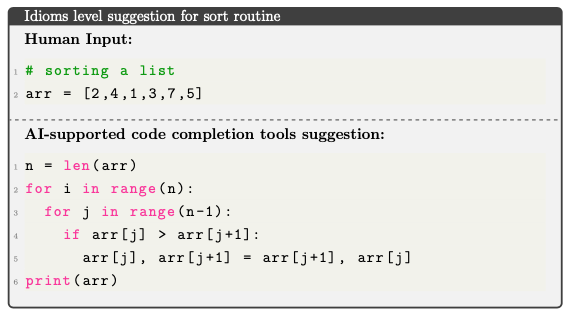
\includegraphics[width=\linewidth]{Figures/idioms.png}
    \caption{Code suggestion of \cct{} at paradigms and idioms level}
    \label{fig:idioms}
\end{figure}

The goal of this software abstraction level in the taxonomy is for \cct{} to be able to detect and use commonly known idiomatic approaches and paradigms that occur in public code in its code suggestions for suggesting code to solve a programming task.

The capabilities required by \cct{} to satisfy paradigms and idioms level of software abstraction are as follows:
\begin{enumerate}
    \item Identify common patterns like paradigms and language idioms in public code repositories~(training data).
    \item Use paradigms and language idioms in suggesting solutions for a programming task.
    \item Satisfy requirements of all the levels below paradigms and idioms in our taxonomy.
\end{enumerate}

% \begin{tcolorbox}[title=Idioms level suggestion for sort routine,boxsep=.15mm]
%     %https://tex.stackexchange.com/questions/337909/tcolorbox-tcbline-style
% \textbf{Human Input:}
% \begin{lstlisting}[language={Python}]
% # sorting a list
% arr = [2,4,1,3,7,5]
% \end{lstlisting}
% \tcbline
% \textbf{\cct{} suggestion:}
% \begin{lstlisting}[language={Python}]
% n = len(arr)
% for i in range(n):
% 	for j in range(n-1):
% 		if arr[j] > arr[j+1]:
% 			arr[j], arr[j+1] = arr[j+1], arr[j]
% print(arr)
% \end{lstlisting}
% \end{tcolorbox}